\documentclass[../mathNotesPreamble]{subfiles}

\begin{document}
% \relscale{1.4} %TODO
  \section{2.1: Functions and Their Graphs}
  \begin{defn*}
    A \textbf{function} is a rule that assigns to each element in a set $A$ one and only one element in a set $B$.

    In the context above, the set $A$ is called the \textbf{domain}, and the set $B$ is called the \textbf{range}.
  \end{defn*}

  \noindent
  \begin{minipage}{0.495\linewidth}
    \newcommand{\funcMachine}{--++(0,-vert) --++(dx,-dy) |- ++(-a,-vert) |- ++(c,-h)
      -- ++(0,-vert) --++(-dx, -dy)[sharp corners] --++(0,-vert-vgap) %bottom left portion
      --++(b+2*dx,0)[rounded corners] --++(0,vert+vgap) --++(-dx,dy) |- ++(a,vert)
      -- ++(0,h) -| ++(-c,vert) --++(dx,dy) --++(0,vert); %top right portion
    }
    \centering
    %bottom left corner is (0,0)
    %a,b,c are widths representing left wall to chute, width of chute, chute to right wall
    %h is height of rectangle
    %dx, dy control slope of "funnel"
    %vert is the height of straight parts of "funnel"
    %paths start at top left (on "funnel")
    \begin{tikzpicture}[declare function={
      a=1.25; b=1.25; c=5.5;
      dx=0.9*a; dy=0.6*a;
      h=1.75; vert=0.6; vgap=0.2;}]
      \begin{scope}
        \clip (-0.1+0,h+2*vert+dy) rectangle ++(0.2+a+b+c,-4*vert-2*dy-h);
        \draw[line width=1pt, fill=lander_blue!25, rounded corners=6pt]
          (a-dx,h+2*vert+dy) \funcMachine
      \end{scope}
      \node (Input) [align=center] at ({a+b/2},{h+vert+dy}) {Input\\$x$};
      \node[align=center] at ({(a+b+c)/2},{h/2}) {$f$};
      \node (Output) [align=center] at ({c+b/2},{-vert-dy}) {$f(x)$\\Output};

      \draw[->] (Input) -- ++(0,-vert-dy);
      \draw[<-] (Output) -- ++(0,vert+dy);
    \end{tikzpicture}
  \end{minipage}\hfill%
  \begin{minipage}{0.495\linewidth}
    \begin{center}
      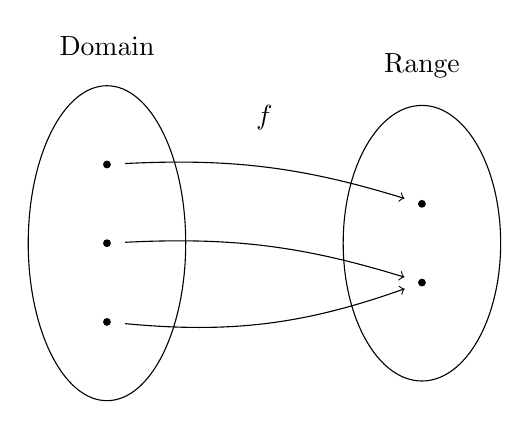
\begin{tikzpicture}
        \draw (-2,0) circle [x radius=1, y radius=2];
        \node at (-2,2.5) {Domain};
        \draw (2,0) circle [x radius=1, y radius=1.75];
        \node at (2,2.25) {Range};
        \node[circle, fill, inner sep=1pt] (xo) at (-2,1) {};
        \node[circle, fill, inner sep=1pt] (fxo) at (2,0.5) {};
        \node[circle, fill, inner sep=1pt] (xt) at (-2,0) {};
        \node[circle, fill, inner sep=1pt] (xr) at (-2,-1) {};
        \node[circle, fill, inner sep=1pt] (fxt) at (2,-0.5) {};
        \node at (0,1.6) {$f$};
        \draw[->, shorten >=5pt, shorten <=5pt] (xo) to [bend left=10] (fxo);
        \draw[->, shorten >=5pt, shorten <=5pt] (xt) to [bend left=10] (fxt);
        \draw[->, shorten >=5pt, shorten <=5pt] (xr) to [bend right=12.5] (fxt);
      \end{tikzpicture}
    \end{center}
  \end{minipage}

  \begin{ex*}
    Let $f(x)=2x^2-2x+1$. Evaluate the following
  \end{ex*}
  \begin{extasks}[after-item-skip=\stretch{1}](2)
    \task $f(1)$
    \task $f(-2)$
    \task $f(a)$
    \task $f(a+h)$
  \end{extasks}
  \vspace*{\stretch{1}}
  \pagebreak

  \begin{ex*}
    Find the domain and range of the following functions:
  \end{ex*}
  \begin{extasks}[after-item-skip=\stretch{1}](2)
    \task $f(x)=x$
    \task $A=\pi r^2$
    \task $y=\sqrt{x-1}$
    \task $y=\dfrac{1}{x^2-4}$
  \end{extasks}
  \vspace*{\stretch{1}}
  \pagebreak

  \begin{ex*}
    An open box is to be made from a rectangular piece of cardboard 16 inches long and 10 inches wide by cutting away identical squares ($x$ inches by $x$ inches) from each corner and folding up the resulting flaps. Find an expression that gives the volume $V$ of the box as a function of $x$. What is the domain of the function?
  \end{ex*}
  \vspace*{0.5\baselineskip}

  \noindent
  \begin{minipage}{0.525\linewidth}
    \begin{tikzpicture}[scale=0.5,
      declare function={
      x=10/3.75;
      hgt=10-2*x;
      wdth=16-2*x;}]
        \coordinate (A) at (x,0);
        \coordinate (B) at (x+wdth,0);
        \coordinate (C) at (2*x+wdth,x);
        \coordinate (D) at (2*x+wdth,x+hgt);
        \coordinate (E) at (x+wdth,2*x+hgt);
        \coordinate (F) at (x,2*x+hgt);
        \coordinate (G) at (0,x+hgt);
        \coordinate (H) at (0,x);

       \shade[shading=radial, inner color= white, outer color=gray!10] (0,0) rectangle (2*x+wdth,2*x+hgt);
       \draw[densely dotted,line width=0.65pt]
         ($(A)+(0,x)$)--($(F)+(0,-x)$)
         ($(B)+(0,x)$)--($(E)+(0,-x)$)
         ($(C)-(x,0)$)--($(H)+(x,0)$)
         ($(D)-(x,0)$)--($(G)+(x,0)$);
       \draw[densely dashed, line width=0.65pt]
         (H)|-(A) (B)-|(C) (D)|-(E) (F)-|(G);
       \draw[line width=1.0pt, fill=white] (A)--(B)|-(C)--(D)-|(E)--(F)|-node[right, pos=0.25] {$x$} node[below, pos=0.75] {$x$} (G)--(H)-|cycle;
       \draw[decorate, decoration={brace, amplitude=15pt}] ($(H)-(10pt,x)$)--($(G)-(10pt,-x)$) node[pos=0.5, left, xshift=-15pt] {$10$};
       \draw[decorate, decoration={brace, amplitude=15pt}] ($(B)-(-x,10pt)$)--($(A)-(x,10pt)$) node[pos=0.5, below, yshift=-15pt] {$16$};
       \draw[dotted] ($(H)+(x,0)$) -| ($(E)-(0,x)$) -| cycle;
    \end{tikzpicture}
  \end{minipage}\hfill%
  \begin{minipage}{0.45\linewidth}
    \raggedleft
    \begin{tikzpicture}[scale=0.9,
      declare function={
      wdth=4.35; hgt=2;
      x_offset=2.75; y_offset=2.75; brace_spacing=0.15;},
      draw=black, text=black]]
        \coordinate (A) at (0,0);
        \coordinate (B) at (wdth,0);
        \coordinate (C) at (wdth,hgt);
        \coordinate (D) at (0,hgt);
        \coordinate (E) at ($(A)+(x_offset, y_offset)$);
        \coordinate (F) at ($(B)+(x_offset, y_offset)$);
        \coordinate (G) at ($(C)+(x_offset, y_offset)$);
        \coordinate (H) at ($(D)+(x_offset, y_offset)$);

        \draw[line width=1pt] (E)-- (F) -- (G) -- (H) -- cycle;
        \draw[fill=white, line width=1pt] (D) -- (H) -- (E) -- (A) -- cycle;
        \draw[fill=white, line width=1pt] (B) -- (C) -- (G) -- (F) -- cycle;
        \draw[fill=white, line width=1pt] (A) -- (B) -- (C) -- (D) -- cycle;
        \draw[dotted] (A) -- (E) -- (F);% (E) -- ($(C)!(H)!(D)$);

        \draw[decorate, decoration={brace, amplitude=5pt}] ($(A)-(brace_spacing,0)$)--($(D)-(brace_spacing,0)$) node[pos=0.5, left, xshift=-7.5pt, inner sep=0pt] {$x$};
        \draw[decorate, decoration={brace, amplitude=5pt}] ($(B)-(0,brace_spacing)$)--($(A)-(0,brace_spacing)$) node[pos=0.5, below, yshift=-7.5pt, inner sep=0pt] {$10-2x$};
        \draw[decorate, decoration={brace, amplitude=5pt}] ($(F)+(brace_spacing,-brace_spacing)$)--($(B)+(brace_spacing,-brace_spacing)$) node[pos=0.5, below right, yshift=-5pt] {$16-2x$};
    \end{tikzpicture}
  \end{minipage}
  \pagebreak

  \begin{defn*}
    A \textbf{piecewise} function is a function with different definitions for different portions of the domain.
  \end{defn*}
  \begin{ex*}
    Rewrite the following as piecewise functions:
  \end{ex*}
  \begin{extasks}[after-item-skip=\stretch{1}](2)
    \task $\abs{x}=$
    \task $\dfrac{x}{\abs{x}}=$
    \task $\abs{x-1}+\abs{4-x}=$
  \end{extasks}
  \vspace*{\stretch{1}}
  \pagebreak

  \begin{defn*}[Vertical Line Test]
    A curve in the $xy$-plane is the graph of a function $y=f(x)$ (an explicit function) if and only if each vertical line intersects it in at most one point
  \end{defn*}
  \begin{ex*}
    Use the vertical line test on the following graphs to determine which graphs may represent an explicit function:
  \end{ex*}

  \begin{center}
    \begin{tabular}{c@{\hspace*{40pt}}c}
      \begin{tikzpicture}[declare function={
        f(\x)=(\x-1.5)*(\x+1)*(\x+2)+6;}]
        \begin{axis}[
          axis lines=center,
          axis line style={black,->},
          xmajorticks=false,
          ymajorticks=false,
          xmin=-3.25, xmax=3.25,
          enlargelimits={value=0.025, auto},
          ticklabel style={font=\footnotesize,inner sep=0.5pt,fill=white,opacity=1.0, text opacity=1},
          xlabel=$x$, xlabel style={at={(ticklabel* cs:1)},anchor=north west},
          ylabel=$y$, ylabel style={at={(ticklabel* cs:1)},anchor=south west},
          every axis plot/.append style={domain=xmin:xmax, line width=0.95pt, color=lander_blue, samples=255},
          ]
          \addplot[<->] expression[domain=-3:2.25]{f(x)};
        \end{axis}
      \end{tikzpicture} &
      \begin{tikzpicture}
        \begin{axis}[
          axis lines=center,
          axis line style={black,->},
          xmajorticks=false,
          ymajorticks=false,
          xmin=-4, xmax=4,
          ymin=-1, ymax=5,
          enlargelimits={value=0.025, auto},
          ticklabel style={font=\footnotesize,inner sep=0.5pt,fill=white,opacity=1.0, text opacity=1},
          xlabel=$x$, xlabel style={at={(ticklabel* cs:1)},anchor=north west},
          ylabel=$y$, ylabel style={at={(ticklabel* cs:1)},anchor=south west},
          every axis plot/.append style={domain=xmin:xmax, line width=0.95pt, color=lander_blue, samples=255},
          ]
          \draw[samples=255, line width=0.95pt, lander_blue, domain=0.2:3.8, <->] plot({(\x-1)*(\x-2)*(\x-3)},{\x});
        \end{axis}
      \end{tikzpicture}\\[2\baselineskip]
      \begin{tikzpicture}[declare function={
        f(\x)=sqrt(\x^2-1);}]
        \begin{axis}[
          axis lines=center,
          axis line style={black,->},
          xmajorticks=false,
          ymajorticks=false,
          ymax=10,
          enlargelimits={value=0.025, auto},
          ticklabel style={font=\footnotesize,inner sep=0.5pt,fill=white,opacity=1.0, text opacity=1},
          xlabel=$x$, xlabel style={at={(ticklabel* cs:1)},anchor=north west},
          ylabel=$y$, ylabel style={at={(ticklabel* cs:1)},anchor=south west},
          every axis plot/.append style={domain=xmin:xmax, line width=0.95pt, color=lander_blue, samples=255},
          ]
          \addplot[<-] expression[domain=-5:-1]{f(x)};
          \addplot[->] expression[domain=1:5]{f(x)};
        \end{axis}
      \end{tikzpicture}&
      \begin{tikzpicture}[declare function={
        g(\x)=1.25*(abs(\x)-1);
        f(\x)=g(\x)<=0 ? sqrt(1-x^2) : g(\x);}]
        \begin{axis}[
          axis lines=center,
          axis equal,
          axis line style={black,->},
          xmajorticks=false,
          ymajorticks=false,
          enlargelimits={value=0.025, auto},
          ticklabel style={font=\footnotesize,inner sep=0.5pt,fill=white,opacity=1.0, text opacity=1},
          xlabel=$x$, xlabel style={at={(ticklabel* cs:1)},anchor=north west},
          ylabel=$y$, ylabel style={at={(ticklabel* cs:1)},anchor=south west},
          every axis plot/.append style={domain=xmin:xmax, line width=0.95pt, color=lander_blue, samples=255},
          ]
          \addplot[<->] expression[domain=-2:2, samples=511]{f(x)};
        \end{axis}
      \end{tikzpicture}
    \end{tabular}
  \end{center}

  \pagebreak
\end{document}
